\chapter{Results and Discussion}
\label{ch:results}

Every number in this chapter comes from a file or a command in the repository, or from one of the scripts {\small\path{thesis/experiments/rq2_experiments.py}} and {\small\path{thesis_amrita/experiments/cap_sweep.py}}. All data are synthetic. Where a result is weak we say so in the same paragraph that reports it.

\section{Evaluation Setup and Metrics}
Since no real procurement or typing data was available, each engine is evaluated on data produced by a generator with a fixed random seed. This makes every experiment repeatable, but it also means that the results describe the engine under the generator's assumptions. The measures used are the following.

\begin{itemize}
    \item \textbf{False-alarm rate}: the share of genuine cases that are flagged. For the keystroke detector this is the share of human sessions with risk at or above 50.
    \item \textbf{Detection rate}: the share of attack cases that are flagged. The macro detection rate is the unweighted mean over the three core attack types, so that no single attack dominates.
    \item \textbf{ROC-AUC}: the probability that a randomly chosen attack session receives a higher risk score than a randomly chosen human session \cite{fawcett2006roc}. It summarises ranking quality independent of any threshold.
    \item \textbf{Wilson interval}: the 95\% confidence interval for a proportion, used for the detection and false-alarm rates because it behaves sensibly near 0 and 1 \cite{wilson1927probable}.
\end{itemize}

\section{Test Suites}
We ran the suites on the final repository (Windows, Python 3.13). Table~\ref{tab:tests} gives the outcome.

\begin{table}[htbp]
\centering
\caption{Automated test results on the final repository}
\label{tab:tests}
\small
\begin{tabularx}{\textwidth}{@{}>{\raggedright\arraybackslash}p{4.4cm}>{\raggedright\arraybackslash}X@{}}
\toprule
\textbf{Suite} & \textbf{Result} \\
\midrule
Cartel, solvency, trust optimizer & 21 passed \\
Backend gateway & 162 passed, 5 failed, 4 skipped \\
Biometrics engine & 219 passed (the browser test and two modules needing \texttt{pytest-asyncio} were excluded from this run) \\
\bottomrule
\end{tabularx}
\end{table}

The five backend failures are one test in \texttt{test\_rule\_retrieval.py} and four in \texttt{test\_vendor\_portal.py}. The first expects an error when both language-model providers fail, but the extractor now falls back to the regular-expression parser, so the test is out of date. In the other four, which concern the shipped bidder pool and IP fields, the cause was not diagnosed; they may depend on state in the local database. We report them as failures and do not hide them.

\section{Keystroke Detector (RQ3)}
\label{sec:res_bio_len}
The protocol is in \texttt{engines/biometrics/reports/evaluation\_report.md} \cite{bioreport}. A generator with seed 42 produced 39{,}000 sessions of 10--300 keystrokes, with lengths drawn log-uniformly so that short and long sessions are both common. Genuine humans (typical, fast and slow typists) were split 60/25/15 into training, calibration and test by session; bots appear only in evaluation. The four bot classes differ in how closely they imitate a person. A regular script types at a perfectly even rhythm. Burst injection sends small chunks of characters separated by pauses. The adaptive bot varies its timing to look human, and its hold times are the main thing that betrays it (see the flight-only result below). The mimic bot is a stress test that copies the mean, spread and pause rate of human typing. Table~\ref{tab:bio} shows the full model.

\begin{table}[htbp]
\centering
\caption{Full-model detection at risk $\ge 50$ (95\% Wilson intervals)}
\label{tab:bio}
\small
\begin{tabular}{@{}lrl@{}}
\toprule
\textbf{Class} & \textbf{Sessions} & \textbf{Flagged} \\
\midrule
Genuine humans (all three styles) & 2700 & 4.6\% (3.8--5.4) \\
Regular script & 6000 & 100.0\% (99.9--100) \\
Burst injection & 6000 & 100.0\% (99.9--100) \\
Adaptive bot & 6000 & 54.6\% (53.4--55.9) \\
Mimic bot (stress test) & 3000 & 44.7\% (42.9--46.5) \\
\midrule
Macro detection (three core attacks) & & 84.9\% \\
ROC-AUC (core attacks vs.\ humans) & & 0.958 (0.955--0.960) \\
\bottomrule
\end{tabular}
\end{table}

Detection of the adaptive bot depends strongly on session length (Figure~\ref{fig:biolen}): 13\% for 10--19 keystrokes, 40\% for 30--49, 92\% for 100--199 and 98\% for 200--300. The figure shows four of the six length bands; the other two, 20--29 and 50--99 keystrokes, give 24\% and 68\%. A short session simply carries too little evidence, and it also raises false alarms on humans: 7.5\% of genuine sessions of 10--19 keystrokes are flagged, against 2.4\% at 200--300, so the length-band thresholds of Section~\ref{sec:bio} do not equalise the false-alarm rate across lengths. In flight-only mode the human false-alarm rate is unchanged at 4.6\%, but macro detection drops to 67.3\% and the adaptive bot is almost invisible (1.9\%), because without hold times it cannot be told apart from a human.

\begin{figure}[htbp]
\centering
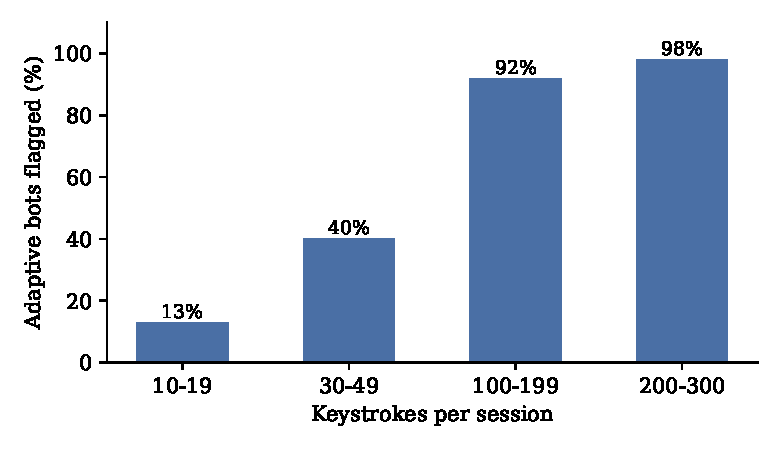
\includegraphics[width=0.72\textwidth]{fig_bio_length.pdf}
\caption{Share of adaptive-bot sessions flagged at risk $\ge 50$, by session length (full model).}
\label{fig:biolen}
\end{figure}

Table~\ref{tab:cmp} compares the shipped mixture with the Isolation Forest of the first design, both calibrated to the same false-alarm budget on the same data.

\begin{table}[htbp]
\centering
\caption{Detector comparison, full mode, same data and false-alarm budget}
\label{tab:cmp}
\small
\begin{tabular}{@{}lrrrr@{}}
\toprule
\textbf{Detector} & \textbf{Adaptive} & \textbf{Mimic} & \textbf{Macro} & \textbf{AUC} \\
\midrule
Gaussian mixture (shipped) & 54.6\% & 44.7\% & 84.9\% & 0.958 \\
Isolation Forest, PCA-whitened & 47.3\% & 19.4\% & 82.4\% & 0.951 \\
Isolation Forest, standardised only & 2.4\% & 4.0\% & 67.5\% & 0.897 \\
\bottomrule
\end{tabular}
\end{table}

The comparison shows that preprocessing mattered as much as the choice of detector. The same Isolation Forest that nearly misses the adaptive bot (2.4\%) when features are only standardised reaches 47.3\% after PCA whitening, close to the mixture. The mixture was kept because it was ahead on every column and because it can be exported as plain parameters.

\paragraph{Limits.} When bots are rare a flag is weak evidence: at a 1\% share of automated sessions the precision of a risk-50 flag is 15.8\%, which is why the output is advisory. A held-out typing style is the larger risk: when one human style was withheld from training and calibration, 51--81\% of its sessions were flagged. The model treats the training population as normal, and real deployment would require retraining on real bidders. The scoring latency measured on an AMD64 machine under Windows is a p95 of 0.54 ms in process and 3.4 ms through an in-process ASGI call, within the 15 ms target but excluding network time.

These results support RQ3 for synthetic sessions only. They show that timing separates crude automation from human typing, and that it is much weaker against bots that imitate human timing.

\section{Ledger Repair (RQ2)}
\label{sec:res_ledger}
We generated 500 statements of 40 rows for each of three conditions, with integer rupee amounts and a valid recurrence. In the OCR condition one balance digit was replaced by its confusable partner. In the tamper condition one balance was inflated by Rs~5{,}000--2{,}00{,}000. The strict check applies the recurrence with no repair; the lattice check is the engine's row verifier. Table~\ref{tab:ledger} shows the number of statements flagged.

\begin{table}[htbp]
\centering
\caption{Statements flagged out of 500 per condition}
\label{tab:ledger}
\small
\begin{tabular}{@{}lrr@{}}
\toprule
\textbf{Condition} & \textbf{Strict recurrence} & \textbf{With OCR lattice} \\
\midrule
Clean & 0 & 0 \\
Scanning noise (benign) & 500 & 17 \\
Tampered balance & 500 & 500 \\
\bottomrule
\end{tabular}
\end{table}

The lattice cleared 483 of 500 noisy statements (96.6\%) and missed none of the 500 tampered ones. Without it, a strict check would send every scanned statement to a human, which is the practical argument for the repair step.

The 17 remaining noise cases were not traced individually; the cause was traced on a separate sample (36 of 1000): the search accepts the first combination that satisfies the recurrence, and sometimes that combination changes the credit or debit and not the corrupted balance. The corrupted balance is then carried forward and the next row fails, so the statement is still flagged, but at the wrong row. This is a weakness in how the repair is attributed. A tampering that happens to equal a confusion swap could be explained away in the same manner, although none of the 500 random inflations was. This result is also easier than it looks: the inflations were drawn at random, so only a small share of them could coincide with a single-digit confusion swap (a 1 changed to a 7 in the thousands place, for example, adds exactly Rs~6{,}000), and 500 of 500 is close to the expected outcome. A forger who edits with confusable digits was not tested, and that is the case in which the repair step could excuse a real forgery. The simulation is also simple (one error per statement, uniform amounts), so the real rate will differ.

\section{Cartel Graph (RQ2)}
Each of 300 synthetic pools has exactly 12 bidders (66 pairs) with unique directors and assets, an IP chosen from three shared addresses and a bank code from four shared codes, as when firms use a common provider and branches. In 120 pools three random bidders also share one director (a planted ring). A naive method flags every pair sharing any attribute; the engine's \texttt{build\_cartel\_summary} is compared with it. A pool with a planted ring has $66-3=63$ honest pairs and one without has 66, so the total is $120\times63+180\times66=19{,}440$ honest pairs.

\begin{table}[htbp]
\centering
\caption{Cartel experiment at the default cap: 300 pools, 19{,}440 honest bidder pairs}
\label{tab:cartel}
\small
\begin{tabular}{@{}lr@{}}
\toprule
\textbf{Measure} & \textbf{Value} \\
\midrule
Honest pairs flagged, naive method & 9{,}655 \\
Honest pairs flagged, engine & 6{,}771 (29.9\% fewer) \\
Planted rings fully recovered & 120 of 120 \\
Mean anomaly score, ring members & 0.320 \\
Mean anomaly score, other bidders & 0.093 \\
\bottomrule
\end{tabular}
\end{table}

The engine never missed a ring, and ring members score about three times higher than other bidders. The reduction in false pairs is modest at the default cap. With 12 bidders over 3 addresses each address is shared by four firms on average, so the cap, which applies only to groups of more than five, affects only the larger random groups and removes only part of the false pairs. The sweep below shows how much of the result depends on that one parameter.

\subsection{Sensitivity to the public-infrastructure cap}
To see how much of the result is a consequence of the cap, we repeated the experiment with the cap set to 2, 3, 4, 5, 6 and 8, using the environment variable \texttt{AEGIS\_PUBLIC\_DEGREE\_CAP} and the same pools. The results are in Table~\ref{tab:cap} and Figure~\ref{fig:cap}.

\begin{table}[htbp]
\centering
\caption{Honest pairs flagged by the engine for different caps (naive method: 9{,}655)}
\label{tab:cap}
\small
\begin{tabular}{@{}lrrr@{}}
\toprule
\textbf{Cap} & \textbf{Honest pairs flagged} & \textbf{Reduction vs.\ naive} & \textbf{Rings recovered} \\
\midrule
2 & 375 & 96.1\% & 120 of 120 \\
3 & 1{,}877 & 80.6\% & 120 of 120 \\
4 & 4{,}199 & 56.5\% & 120 of 120 \\
5 (default) & 6{,}771 & 29.9\% & 120 of 120 \\
6 & 8{,}356 & 13.5\% & 120 of 120 \\
8 & 9{,}532 & 1.3\% & 120 of 120 \\
\bottomrule
\end{tabular}
\end{table}

\begin{figure}[htbp]
\centering
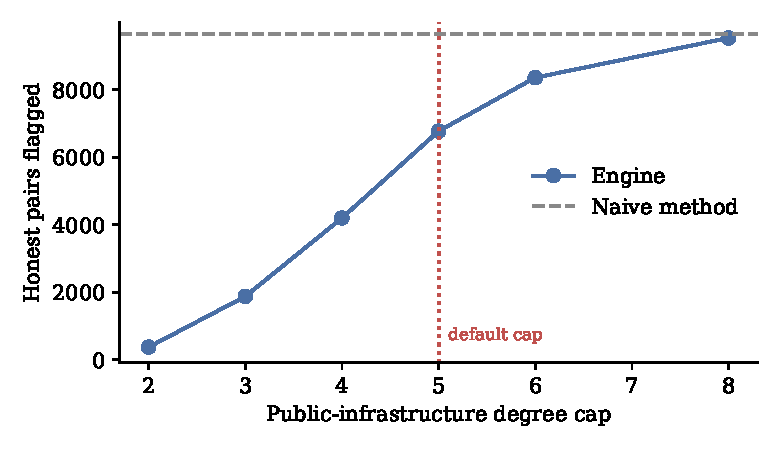
\includegraphics[width=0.72\textwidth]{fig_cap_sweep.pdf}
\caption{False pairs flagged by the engine as the public-infrastructure cap varies.}
\label{fig:cap}
\end{figure}

The 29.9\% reduction is therefore a property of the cap, not of the engine. The degree-discounted weight $w(d)$ does not enter the pair flag at all, so it plays no part in this reduction. A cap of 3 removes about four fifths of the false pairs here, and a cap of 8 removes almost none. Ring recovery stays perfect at every setting, but this must not be over-read. The planted rings are linked by a shared director, and directors are never capped, so lowering the cap cannot hurt recall in this experiment by construction. In real data a ring that shared only an IP address or a bank branch would be hidden by a low cap. The experiment cannot measure that cost, and the right cap has to be chosen on real bidder data, with the trade-off between nuisance flags and missed rings made explicitly. The pair list also still needs the anomaly score to be useful. Even at the default cap the engine flags 6{,}771 of 19{,}440 honest pairs (34.8\%), and the 29.9\% figure is measured against a deliberately naive baseline, so the experiment does not show a useful false-alarm rate on real bidders.

\section{Trust Optimizer Simulation}
The bundled simulation (\texttt{run\_simulation.py}, seed 42) ranks 20 bidders for one tender. The two colluders have anomaly 0.833 and are both excluded, but not by the collusion penalty: both fail the technical minimum (a technical score of 0.2324 against a threshold of about 0.3), and the penalty $\mu A_i$ would only have lowered their composite score by about 0.25. In this run the anomaly score therefore did not decide the outcome. Only 7 of the 20 bidders pass the gates, and the winner, B020, has a fused trust of 0.8376 and a price score of 1.17. A bidder with a very low price but the lowest financial score is stopped by the eligibility gate, and a bidder that under-declared litigation receives a legal score of 0.0012. The winner's trust becomes 0.8700 after a successful project and 0.6700 after a failed one. These are constructed cases, not an accuracy measurement. They show the eligibility gate, the legal penalty and the trust update acting on cases built to trigger them. They do not show the collusion penalty $\mu A_i$ changing an outcome, so that safeguard remains untested in this thesis.

\section{Tender Pipeline (RQ1)}
The project README reports an end-to-end run on a real GeM tender whose extracted EMD, turnover (Rs~27 lakh), experience (three years) and MSE exemption match the document. We did not repeat it for this thesis, since it needs a model key, so it is reported as anecdotal. The unit tests check CDS values, exemption handling and the orchestrator graph. No experiment here measures how often the extractor is wrong or how often the symbolic layer catches the error, so RQ1 is supported by design and tests but not by an error-rate study.

\section{Discussion and Threats to Validity}
The biometrics engine has the most extensive evaluation here (the largest sample, confidence intervals and a baseline comparison), but all of it is synthetic, so none of the engines is validated on real data. The main threats are:
\begin{itemize}
    \item \textbf{Synthetic data.} Detector and experiment results depend on the generators that the project authors wrote, and the mixture size was chosen on a development set built from the same generator. They show behaviour under stated assumptions, not field accuracy.
    \item \textbf{Own experiments.} We wrote the ledger and cartel experiments to test the safeguards, so they may favour the design. The cap sweep partly guards against this, since it shows a setting where the safeguard looks weak.
    \item \textbf{Untested paths.} The scanned-PDF OCR route and live Gemini extraction were not exercised here, and five tests fail.
    \item \textbf{Single seeds.} The experiments use one seed each. The Wilson intervals describe sampling error within a seed, not variation between generators.
\end{itemize}

Taken together, the results say something consistent. The safeguards work in the direction intended, although their cost (for example the wrongly cleared forgeries or missed rings they may cause on real data) was not measured, and each one has a parameter or an assumption that decides how much it helps: the cap in the cartel graph, the single-error assumption in the ledger repair, and the session length for the keystroke detector. A reader who wants to rely on any of these engines should treat the parameter as the thing to calibrate first.
